\chapter{Metodología}

Además del desarrollo de la plataforma de la aeronave, otro objetivo del trabajo es intentar estabilizar un UAV usando algoritmos de control basados en algoritmos de aprendizaje automático.En este apartado, se tratará sobre la metodología que se ha llevado a cabo durante el proceso de desarrollo de los algoritmos. Los principales componentes que intervienen en el agente son el estado, las acciones y la recompensa, para cada problema hay un conjunto que estados, acciones y funciones de recompensa que pueden llevar a que el agente aprenda.

\section{Diseño del estado}
 El autopiloto cuenta con 2 IMUs para poder obtener datos sobre su estado. Se quiere estabilizar el cuadricóptero en una orientación concreta, por lo tanto el estado que se ha diseñado consta de 6 parámetros:
\begin{equation}
	S=(\varphi,\theta,\psi,\dot\varphi,\dot\theta,\dot\psi) \qquad\qquad \varphi,\theta,\psi,\dot\varphi,\dot\theta,\dot\psi \in [-1,1]
\end{equation} 

Siendo $\varphi,\theta$ y $\psi$ los ángulos de alabeo (\textit{roll}), cabeceo (\textit{pitch}) y guiñada (\textit{yaw}) del cuadricóptero y $\dot\varphi,\dot\theta$ y $\dot\psi$ sus respectivas velocidades. Para favorecer la convergencia del aprendizaje, se ha normalizado el estado para que todas sus componentes estén comprendidas dentro del intervalo $[-1,1]$.

Los ángulos proporcionan información sobre el estado actual y la velocidad angular sobre los estados pasados y los posibles estados futuros, es decir, proporciona cierta información temporal. 

\section{Diseño de las acciones}
Al trabajar con un cuadricóptero podemos actuar sobre la potencia que se le entrega a los motores, por lo que cada acción que realice el agente constará de 4 campos:
\begin{equation}
	A = (T_1,T_2,T_3,T_4) \qquad\qquad T_i \in [-1,1]
\end{equation}

Siendo $T_i$ la potencia \textit{(Thrust)} normalizada entregada a cada motor. Un valor de $T_1=-1$ significa que el motor 1 estaría girando a la mínima potencia permitida y un valor de $T_1=1$ corresponde a que el motor 1 estaría girando a la máxima potencia.\\

Las señales de control que admiten los variadores es una señal PWM de 50Hz cuyo ancho de pulso debe estar entre 1ms y 2ms. Un ancho de pulso de 1ms se corresponde con la mínima velocidad el motor y un ancho de 2ms con la máxima, véase \cref{hardware_ESCWAVE}.\newpage

\begin{figure}[htb!]
	\centering
	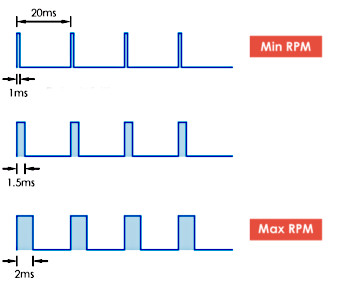
\includegraphics[width=0.6\textwidth]{hardware/ESCWaves}
	\caption{Formas de onda que recibe un variador}
	\label{hardware_ESCWAVE}	
\end{figure}

 Para realizar esta transformación del dominio $[-1,1]$ al dominio [1000,2000] $\mu$s se han empleado la siguiente expresión

\begin{equation}
	P_i= T_i \cdot 1000 \cdot \alpha + \beta \qquad \qquad i=0,...,3
\end{equation}\\
siendo $P_i$ el ancho del pulso enviado al ESC, $\alpha \in [0,1]$  es el porcentaje de la potencia total que puede manejar el controlador y $\beta \in [0,2000]$ es la velocidad base que tienen los motores. Esta velocidad base permite que el cuadricóptero pueda variar su altura y que se pueda autosustentar. 

\section{Diseño de la función de recompensa y ajuste de hiperparámetros}

La búsqueda de la función de recompensa y la elección de los hiperparámetros que aseguraban la convergencia de los distintos algoritmos, se ha realizado mediante un proceso cíclico, en el que, se realizaba una hipótesis sobre la posible forma de la función de recompensa o el posible valor de un hiperparámetro que podría mejorar el algoritmo. Posteriormente se ejecutaba el algoritmo y se comparaban los resultados de este entrenamiento con los resultados previos. Para disminuir el tiempo de los entrenamientos, se simplificaba el problema del control del cuadricóptero a un único eje de giro. Con esto se redujo el tiempo que se tardaba en completar el ciclo.


\subsubsection{Función de recompensa}
La función de recompensa rige la forma en la que la red va a configurar sus pesos, por lo tanto, cómo se va a comportar el agente en un estado determinado. Para conseguir que el agente responda de la forma deseada se han probado una gran variedad de funciones de \textit{reward}, optando finalmente por:
\begin{equation}
	%R_t = \left( 1-\frac{|\varphi - \varphi_{ref}| + |\theta-\theta_{ref}| + |\psi- \psi_{ref}|}{3}\right)^3
	R_t = \left( 1-\frac{|\varphi|  + |\theta| + |\psi|}{3}\right)^n
\end{equation}
Sea $\gamma= \frac{|\varphi|  + |\theta| + |\psi|}{3} $ entonces $R_t = (1- \gamma)^n$, con $n \in \mathbb{N}$. Aumentando el valor de $n$ podemos conseguir funciones de recompensa con pendientes más pronunciadas.

	\begin{figure}[htb!]
\centering
	
	\begin{subfigure}{0.32\textwidth}
		\centering
		\begin{tikzpicture}[]
		\begin{axis}[ 
		%title=$\tanh(x)$,
		domain=0:1, restrict y to domain=-10:10,
		axis x line=middle, xmin=0, xmax=1, xtick={0,0.5,...,1}, xlabel=$\gamma$,
		axis y line=middle, ymin=0, ymax=1, ytick={0,...,1}, ylabel=$r_t$,
		y label style={at={(current axis.below origin)},anchor=south east},
		scale only axis=true,
		width=0.7\textwidth, height=3.5cm,
		samples=40] 
		\addplot[blue, very thick] {(1-(\x))^4};		\end{axis}
		
		%\addlegendentry{$\tanh(x)$}	
		\end{tikzpicture}
	\end{subfigure}
\begin{subfigure}{0.32\textwidth}
	\centering
	\begin{tikzpicture}[]
	\begin{axis}[ 
	%title=$\tanh(x)$,
	domain=0:1, restrict y to domain=-10:10,
	axis x line=middle, xmin=0, xmax=1, xtick={0,0.5,...,1}, xlabel=$\gamma$,
	axis y line=middle, ymin=0, ymax=1, ytick={0,...,1}, ylabel=$r_t$,
	y label style={at={(current axis.below origin)},anchor=south east},
	scale only axis=true,
	width=0.7\textwidth, height=3.5cm,
	samples=40] 
	\addplot[blue, very thick] {(1-(\x))^4};
	\end{axis}
	
	%\addlegendentry{$\tanh(x)$}	
	\end{tikzpicture}
\end{subfigure}
\begin{subfigure}{0.32\textwidth}
	\centering
	\begin{tikzpicture}[]
	\begin{axis}[ 
	%title=$\tanh(x)$,
	domain=0:1, restrict y to domain=-10:10,
	axis x line=middle, xmin=0, xmax=1, xtick={0,0.5,...,1}, xlabel=$\gamma$,
	axis y line=middle, ymin=0, ymax=1, ytick={0,...,1}, ylabel=$r_t$,
	y label style={at={(current axis.below origin)},anchor=south east},
	scale only axis=true,
	width=0.7\textwidth, height=3.5cm,
	samples=40] 
	\addplot[blue, very thick] {(1-(\x))^10};
	\end{axis}
	
	%\addlegendentry{$\tanh(x)$}	
	\end{tikzpicture}
	
\end{subfigure}
	\caption{Funciones $R_t$ para distintos valores de $n = 2,4,10$ respectivamente}
\end{figure}

Esta función $R_t:[0,1]\rightarrow [0,1] \;\; \forall n \in \mathbb{N} > 0$ por lo que al proporcionar valores entre 0 y 1, favorece la velocidad del entrenamiento. Además toda la recompensa es positiva, por lo que el agente intentará mantenerse la mayor cantidad de tiempo posible sin reiniciar el episodio, esto es muy importante para conseguir la convergencia del entrenamiento en los escenarios en los que se desea que el cuadricóptero se encuentre siempre dentro de una región concreta del espacio. 

\subsubsection{Ajuste de hiperparámetros}

Debido a las diferentes naturalezas de cada uno de los algoritmos que se han empleado: DDPG, TRPO y PPO , cada uno cuenta con un conjunto distinto de hiperparámetros que ajustar. La implementación de estos algoritmos que se ha empleado (\textit{stable-baselines}) contiene unos hiperparámetros por defecto, los cuales suelen hacer que los algoritmos converjan.

Por lo general, no ha sido necesario modificar mucho estos parámetros por defecto, a excepción del valor de la constante $\epsilon$ en el algoritmo PPO. Este parámetro modifica el tamaño de la región de confianza del algoritmo, acotando el tamaño de los pasos que se toman en el curso de cada actualización de la política. Se observó que el valor por defecto de este parámetro $\epsilon_{defecto} = 0.2$ era demasiado grande, por lo que la política divergía. A medida que este parámetro se disminuye, se aumenta la estabilidad del aprendizaje, sin embargo, también se ralentiza mucho. Es por esto que el valor de éste hiperpaŕametro se ha ido modificando a lo largo de los experimentos, para poder conseguir el entrenamiento más rápido, capaz de converger de forma estable. 



